\section{Operación}
\label{anexo:operacion}

Tras realizar las verificaciones mencionadas en la Sec. 
\ref{anexo:verificaciones} del Manual de Usuario proceda de la siguiente
manera para la operación normal de la planta.

\subsection{Carga del programa en el PLC}
\label{anexo:operacionPLC}

% \begin{enumerate}
%  \item Controlar el nivel de agua en los tanques según el anexo \ref{anexo:puestaEnMarcha}.
%  \item Controlar que las válvulas manuales estén en su correcta
%  posición según el anexo \ref{anexo:puestaEnMarcha}.
%  \item Conectar el aire a presión según el anexo \ref{anexo:puestaEnMarcha}.
%  \item Conectar la planta a la red eléctrica.
%  \item Activar en interruptor termomagnético ubicado dentro del tablero
%  eléctrico.
%  \item Conectar la planta con la computadora mediante el cable cable RS-485 
%  con adaptación a RS-232. Puede ser necesario utilizar un adaptador RS-232/USB.
%  \item Abrir el programa del \gls{plc} denominado {\color{red}(nombre del programa)} 
%  con el Software Twido Soft. Este programa se encuentra en el DVD adjunto a este 
%  informe.
%  \item Conectarse al \gls{plc} como se indica en la imagen \ref{img:twidosoft}.
%  \item Cargar el programa en el \gls{plc}, imagen \ref{img:twidosoftcargar}.
%  \item Poner a correr el programa, imagen\ref{img:twidosoftrun}.
%  \item Desconectarse del \gls{plc}, imagen \ref{img:twidosoftdesc}.
% \end{enumerate}
Usted puede leer el programa que se encuentra en la memoria del \gls{plc} o bien
para escribir un nuevo programa.
Para esta tarea es necesario que el \gls{plc} se encuentre encendido y
conectado a la computadora que lo programará.
Deberá entonces:

\begin{table}[H]
\centering
\renewcommand*{\arraystretch}{0.01}
\begin{tabular}{*{2}{m{0.44\textwidth}}}
\hline
    Energizar la planta accionando el interruptor
termomagnético ubicado dentro del tablero eléctrico.
    &\begin{center}
      \rule{0.4\textwidth}{0.3\textwidth}
      %\includegraphics[width=0.4\textwidth]
	%{Cap5-SCADA/images/database1.jpeg}
    \end{center}\\
\hline
    Conectar la planta con la computadora de control, mediante el cable cable
\verb|RS-485|  con adaptación a \verb|RS-232|. Puede ser necesario utilizar un
adaptador \verb|RS-232/USB|.
    &\begin{center}
      \rule{0.4\textwidth}{0.3\textwidth}
      %\includegraphics[width=0.4\textwidth]
	%{Cap5-SCADA/images/database1.jpeg}
    \end{center}\\
\hline
\end{tabular}
\end{table}

Procederemos a escribir y ejecutar en el \gls{plc} el programa propuesto en
durante el desarrollo de la planta, así el sistema estará en un estado conocido.
\todo{imagen del programa y colocar el nombre definitivo del programa}
Se debe abrir el programa del \gls{plc} denominado {\color{red}(nombre del
programa)} con el Software Twido Soft. Este programa se encuentra en el DVD 
adjunto a este informe. 
Luego, se debe proceder de la manera que se indica a continuación:

\begin{table}[H]
\centering
\renewcommand*{\arraystretch}{0.01}
\begin{tabular}{*{2}{m{0.45\textwidth}}}
\hline
    En la pantalla principal de TwidoSoft seleccione 
Autómata/Conectar para poder conectarse al \gls{plc}.
    &\begin{center}
      %\rule{0.4\textwidth}{0.3\textwidth}
      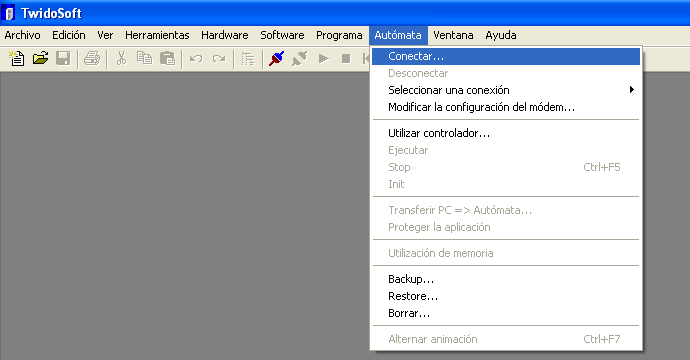
\includegraphics[width=0.4\textwidth]
	{Anexos/images/twidosoft.PNG}
    \end{center}\\
\hline
    Al conectarse, y si existiese una diferencia entre las aplicaciones
de la computadora y el \gls{plc}, el software solicitará en qué sentido debe
realizarse la transferencia de datos.
Cargar el programa desde la computadora al \gls{plc}.
    &\begin{center}
      %\rule{0.4\textwidth}{0.3\textwidth}
      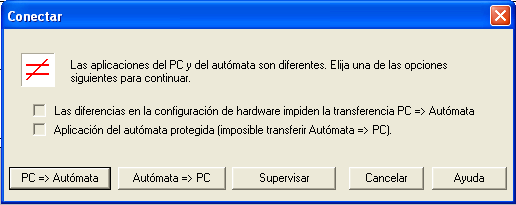
\includegraphics[width=0.4\textwidth]
	{Anexos/images/twidosoftcargar.PNG}
    \end{center}\\
\hline
    Ejecutar el programa, haciendo click el icono \emph{Run}.
    &\begin{center}
      %\rule{0.4\textwidth}{0.3\textwidth}
      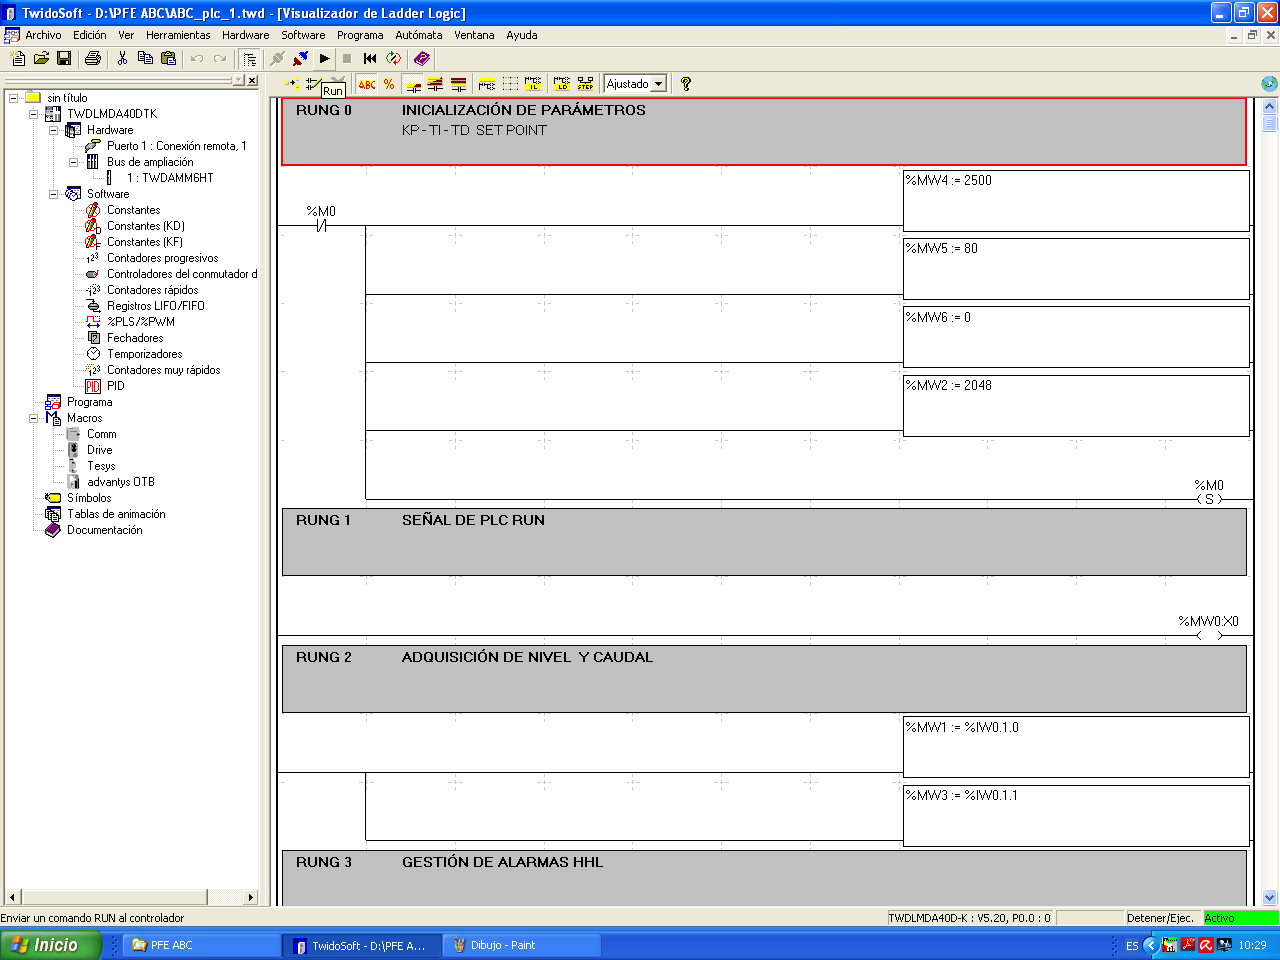
\includegraphics[width=0.4\textwidth]
	{Anexos/images/twidosoftrun.PNG}
    \end{center}\\
\hline
  Finalmente puede desconectarse del \gls{plc}
  &\begin{center}
    %\rule{0.4\textwidth}{0.3\textwidth}
    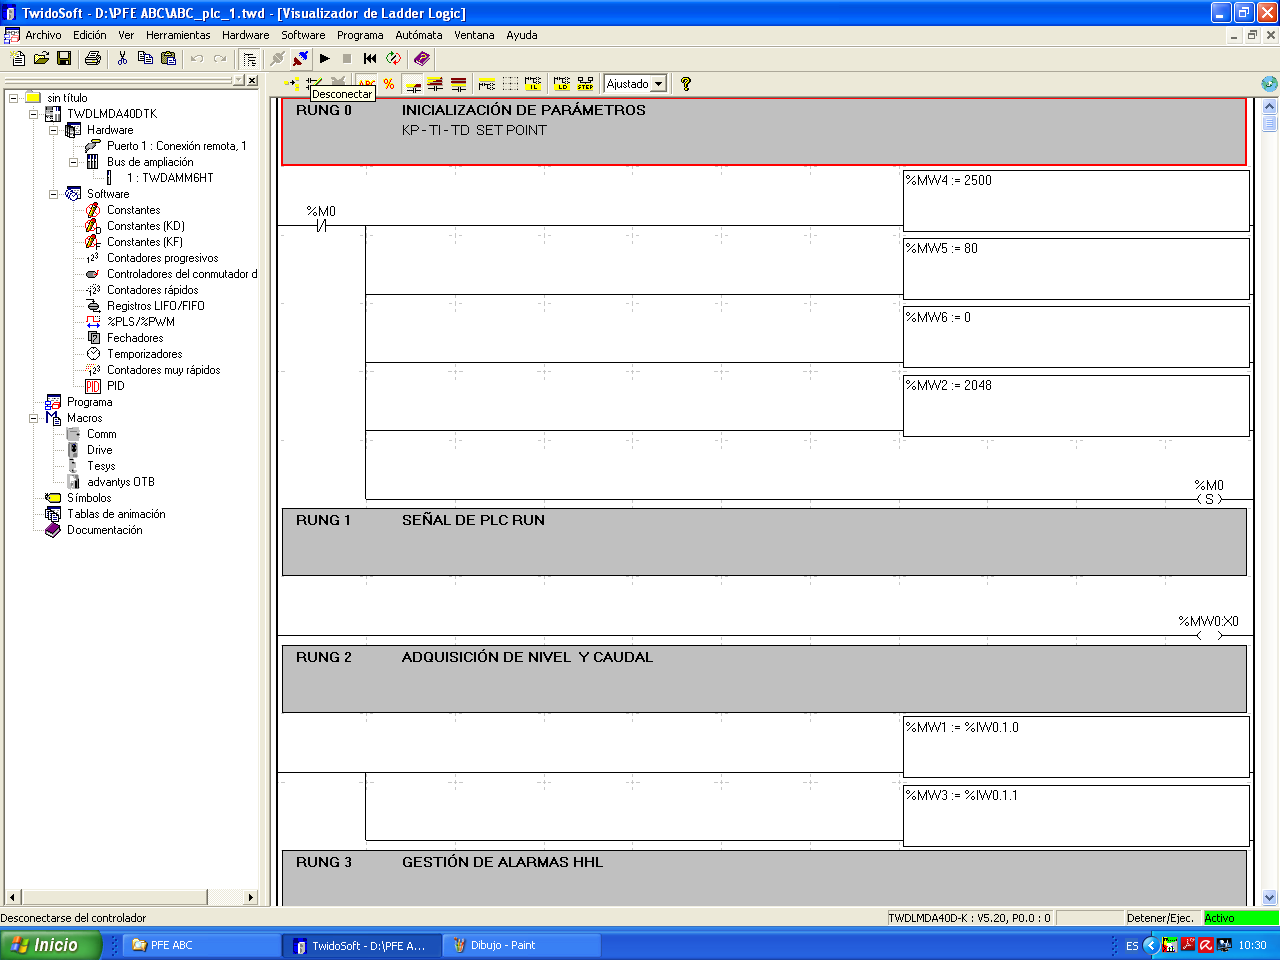
\includegraphics[width=0.4\textwidth]
      {Anexos/images/twidosoftdesc.PNG}
  \end{center}\\
\hline
\end{tabular}
\end{table}


\subsection{SCADA}
Normalmente, si el programa que corre en el \gls{plc} no ha sido cambiado, 
usted debería ser capaz de retomar la operación de la planta desde este punto. 
Para asegurarse de que el programa que corre en el \gls{plc} es el correcto 
refiérase a la Sec. \ref{anexo:operacionPLC} del Manual del Usuario.
\begin{lattention}
 Recuerde siempre realizar las verificaciones descriptas en la Sección 
\ref{anexo:verificaciones} del Manual del Usuario antes de continuar con la
operación de la planta.
\end{lattention}

\subsubsection{Iniciar P-CIM}

Para controlar el sistema desde el \gls{scada} de P-CIM de AFCON, es necesario 
iniciar P-CIM y verificar que el driver de Modbus se haya cargado correctamente:
\begin{table}[!ht]
\centering
\renewcommand*{\arraystretch}{0.01}
\begin{tabular}{*{2}{m{0.45\textwidth}}}
\hline
  Active P-CIM utilizando el Startup de P-CIM del grupo de aplicaciones de la 
carpeta AFCON P-CIM.
  &\begin{center}
    %\rule{0.4\textwidth}{0.3\textwidth}
    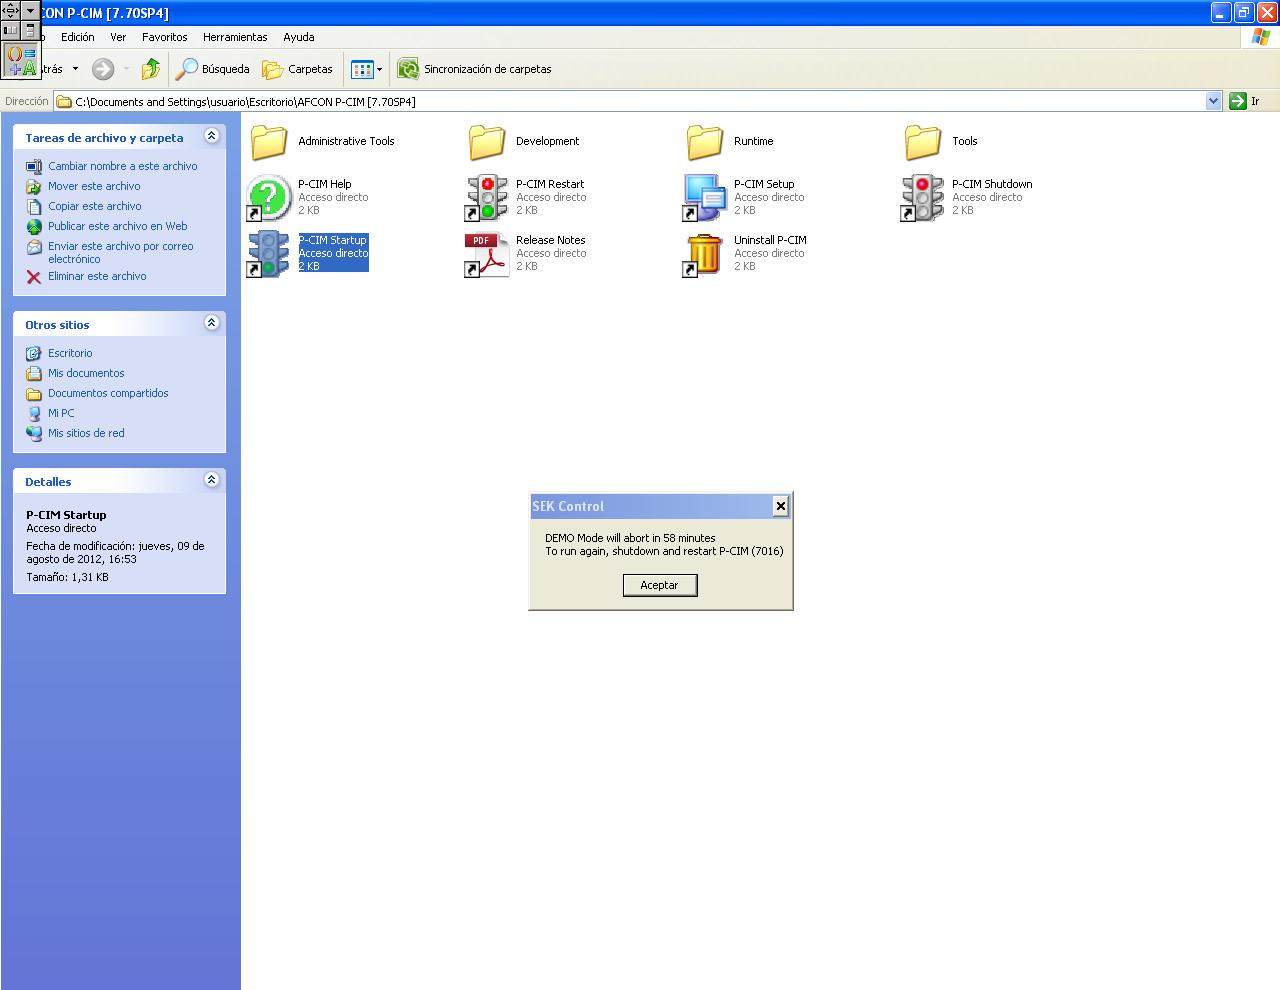
\includegraphics[width=0.4\textwidth]
      {Cap5-SCADA/images/startUp.jpeg}
  \end{center}\\
 \hline
   Verifique que en la ventana Alarm Summary muestre el mensaje “MODBUS
  Driver successfully loaded” indicando que el driver halló la tabla de 
  comunicación y fue exitosamente cargado.
  &\begin{center}
    %\rule{0.4\textwidth}{0.3\textwidth}
    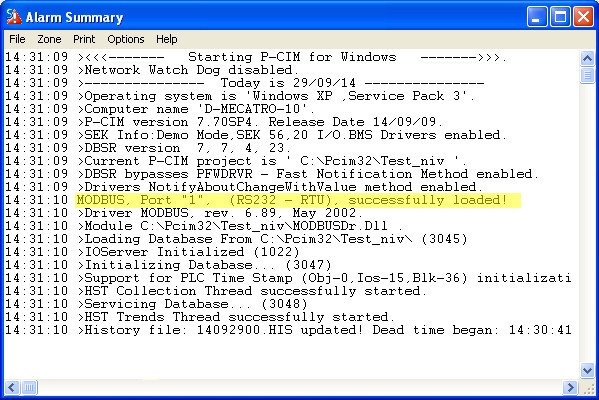
\includegraphics[width=0.4\textwidth]
      {Cap5-SCADA/images/alarm.jpeg}
  \end{center}\\
 \hline
\end{tabular}
\end{table}

\begin{lattention}
En el caso de que no se haya logrado cargar el driver Modbus refiérase a la 
Tab. \ref{tab:PropModbus} de la Sec. \ref{subsubsec:InforDriver} del informe
de proyecto final.
\end{lattention}

\subsubsection{Operators Workspace}

\todo{agregar directorio}
Para ejecutar el entorno gráfico del sistema \gls{scada} abra la aplicación
Operator Workspace que se encuentra en el directorio

A través de esta interfaz es posible manejar la planta.
Pueden diferenciarse 4 bloques principales (Ver Fig.\todo{agregar foto})
\begin{enumerate}
 \item \textbf{Control Automatico:} En esta sección usted puede enviar al
\gls{plc} de la planta la consigna/setpoint y las constantes del controlador
$K_p$, $T_i$ y $T_d$.
 \item \textbf{Control Manual:} Este modo debe ser usado solamente como un
medio para
sacar a la planta de un estado de emergencia tras  haberse declarado una alarma
por HHL o LLL.
Aquí podrá encender las bombas individualmente y controlar la apertura de la
válvula.
 \item \textbf{Sistema:} En este apartado podemos ver el estado del actual del
sistema.
Es decir se muestran los valores de nivel y caudal actuales e históricos juntos
con las alarmas.
 \item \textbf{Activación:} Desde estos controles se activa o detiene la
planta.
\end{enumerate}
